\section{Metodologia}
\label{sec:metodologia}
Neste artigo, é proposto dois diferentes branches. O branch principal (master) onde os desenvolvedores evoluem o projeto e branches secundários, chamados de branches de release, que são as ramificações onde conterá as versões finais (versões de produção) do projeto.
O branch master, usado para a codificação das funcionalidades definidas para a determinada Sprint, sempre conterá o projeto em seu estado de desenvolvimento (versão sufixada com -SNAPSHOT). Após implementadas e testadas tais funcionalidades, perto do final da Sprint, é chegado o momento de gerar uma versão de produção completamente funcional do produto, como descrito em metodologias ágeis. É criado então um branch de release do ponto atual do projeto que originará uma versão de produção. Toda ramificação do branch master para a criação do branch de release, deverá incrementar a versão menor (ou versão maior se for o caso) do projeto, indicando as novas funcionalidades implementadas a partir daquele ponto entrarão em uma outra versão de produção do projeto (geralmente em uma próxima Sprint). Novas versões de correção podem ser lançadas indefinidamente durante o desenvolvimento.
\\\\
Por exemplo: suponhamos que temos um projeto \textbf{FrameworkTeste} na Sprint 2, onde o branch \textbf{master} abriga a versão \textbf{1.2.3-SNAPSHOT} do projeto. Ao fim da Sprint, é criado um branch deste ponto (podemos nomear de rel-1.2) que dará origem à versão final \textbf{1.2.X} do projeto enquanto que o branch \textbf{master} agora passa a abrigar a versão \textbf{1.3.0-SNAPSHOT} que será evoluído no Sprint 3 como pode ser visto na figura \ref{fig:branchingrelease}.

\begin{figure}[h!]
	\centering
	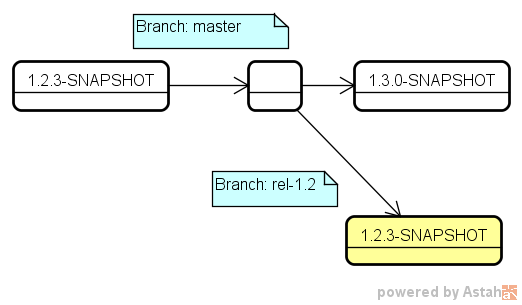
\includegraphics[width=0.7\linewidth]{img/branching_otojr_01}
	\caption[Branching de Release]{Criação do branching de release}
	\label{fig:branchingrelease}
\end{figure}

\subsection{Detalhamento do Branch de Release}
\label{subsec:detalherelease}
Um questionamento comum em relação à ramificação de release é devido ao fato da mesma ser um branch e não um estado fechado (snapshot do SCM) marcado por uma tag. Ou seja, por que utilizar uma ação branch ao invés de uma ação tag?

Apesar de necessário considerar que no ponto de criação do branch da release, o código já tenha passado por todo o ciclo de testes (unidade, regressão, aceitação, etc), é impossível afirmar que o produto a ser lançado está livre de defeitos. Daí o motivo da existência do branch. Este branch é usado para correção de defeitos da release até a "lapidação" da versão final que será entregue ao cliente. 

O mais importante que devemos frisar é que neste branch está proibido adicionar novas funcionalidades para que não ocorra uma regressão de estabilidade no projeto. Neste branch, trabalha-se uma equipe dedicada somente a correção de defeitos. Este ciclo de correção de defeitos pode ocorrer em várias mini-iterações onde que cada iteração seja gerada uma nova versão de correção neste mesmo branch. Cada versão nova de correção deve ser reintegrada novamente ao branch master para que os desenvolvedores  recebam estas correções e o branch principal se mantenha o mais estável possível. 

As iterações de correção ocorrem até que a release esteja em um nível de qualidade acordada e aceitada pelo cliente. Neste momento então, uma versão de produção (não sufixada) deve ser construída, documentada e entregue ao cliente. Opcionalmente pode-se utilizar uma tag para marcar a versão que foi entregue. 

Por exemplo: no projeto FrameworkTeste, versão 1.2.3-SNAPSHOT, é criado o branch de release rel-1.2 onde uma determinada equipe trabalhará com as correções de defeitos. Neste branch, a cada conjunto de defeitos corrigidos, são gerados novas versões 1.2.4, 1.2.5, 1.2.6, até a qualidade aceitada. Neste momento então, digamos que a versão 1.2.6 está apta a ser entregue ao cliente. Esta versão deve ser documentada como versão entregue e opcionalmente podemos marcar como uma tag v1.2.6-Final este ponto da release como mostrado na figura \ref{fig:finalrelease}.

\begin{figure}[h!]
	\centering
	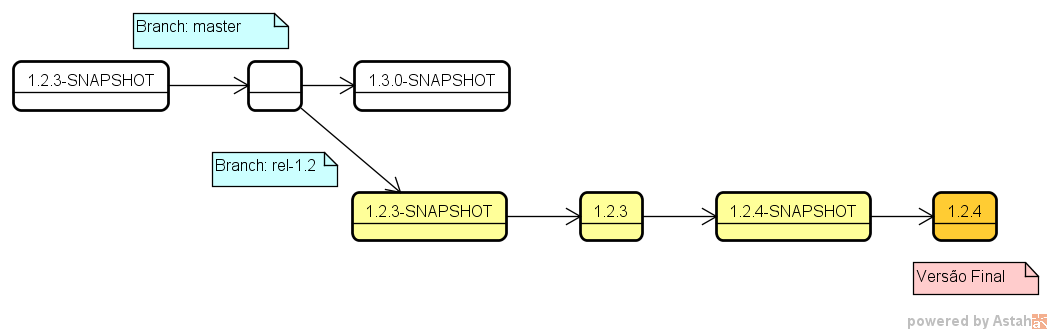
\includegraphics[width=0.7\linewidth]{img/branching_otojr_02}
	\caption[Criação da versão final]{Criação da versão final do produto a partir do branch da release.}
	\label{fig:finalrelease}
\end{figure}

\subsection{Hotfixes}
\label{subsec:hotfixes}
Ocasionalmente, uma versão entregue ao cliente pode apresentar algum defeito. Não é desejável, mas tal situação não é impossível. Neste caso, é necessário que ocorra um Hotfix na versão final entregue. A forma de tratar Hotfixes neste modelo de trabalho proposto ocorre naturalmente no branch de release. É feita mais uma iteração de correção no branch de release e gerada uma nova versão documentada (opcionalmente marcada com tag) como entregue. Pode ser visto na figura \ref{fig:hotfix}

\begin{figure}[h!]
	\centering
	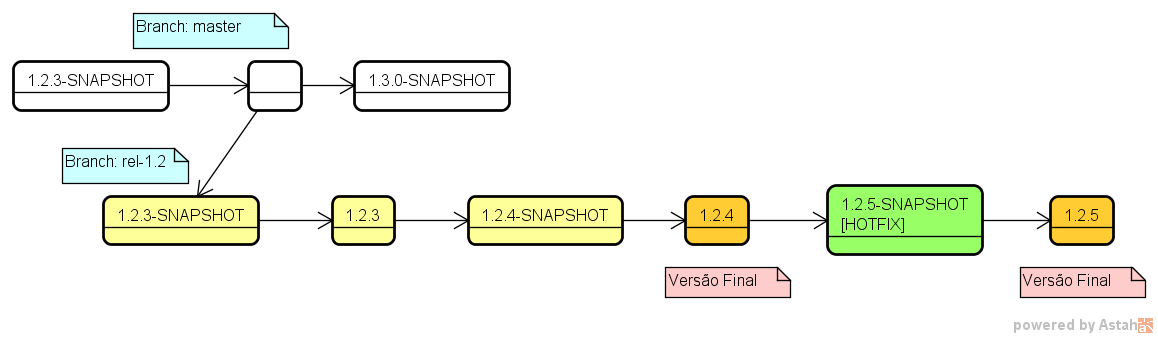
\includegraphics[width=0.7\linewidth]{img/branching_otojr_03}
	\caption[Hotfix na versão final]{Aplicação de um Hotfix na versão final do produto.}
	\label{fig:hotfix}
\end{figure}